\section{Моделирование дискретных распределителей}\label{sec:ch2/sec3}

\subsection{Уравнения массового расхода рабочего тела}\label{sec:ch2/sec3/subsec1}
Массовый расход воздуха через дискретный распределитель
является ключевым параметром, определяющим динамику пневматической
системы. Для его описания используется модель, основанная на уравнении Сен-Венана-Ванцеля:
\begin{equation}
    G = \psi(p_1, p_2) \cdot C_d F_\text{пр} \frac{p_1}{\sqrt{RT_\text{вх}}},
\end{equation}
где
$\psi(p_1, p_2)$ -- расходная функция;
$C_d$ -- коэффициент расхода;
$F_\text{пр}$ -- эффективная площадь проходного сечения;
$p_1$ -- давление на входе;
$p_2$ -- давление на выходе;
$T_\text{вх}$ -- температура воздуха на входе.

Ключевым элементом в данном уравнении является расходная функция $\psi(p_1, p_2)$, которая
учитывает влияние отношения давлений на входе и выходе распределителя
на массовый расход. Эта функция определяется следующим образом:
\begin{equation}
    \psi(p_1, p_2) = \begin{cases}
        \sqrt{\frac{2\gamma}{\gamma-1}\left[\left(\frac{p_2}{p_1}\right)^{\frac{2}{\gamma}} - \left(\frac{p_2}{p_1}\right)^{\frac{\gamma+1}{\gamma}}\right]}, & \text{если } \frac{p_2}{p_1} > b_{кр}    \\
        \sqrt{\gamma \left(\frac{2}{\gamma+1}\right)^{\frac{\gamma+1}{\gamma-1}}},                                                                            & \text{если } \frac{p_2}{p_1} \leq b_{кр}
    \end{cases}
\end{equation}
где
$b_{кр} = \left(\frac{2}{\gamma+1}\right)^{\frac{\gamma}{\gamma-1}}$ -- критическое отношение давлений.

Для наглядного представления характера изменения расходной функции
$\psi(p_1, p_2)$ в зависимости от отношения давлений $p_2/p_1$
приведен график представлены на рисунке \ref{fig:ch2/mass_flow_function}.
\begin{figure}
    \centerfloat{
        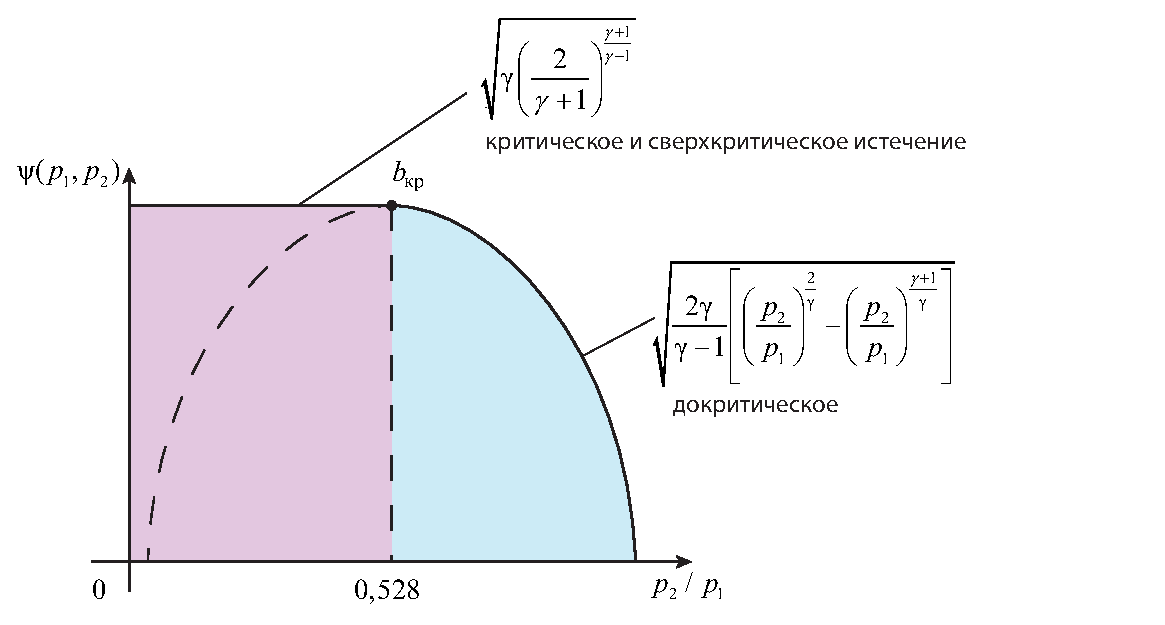
\includegraphics{part2/critical_gas_flow_chart.eps}
    }
    \caption{График расходной функции $\psi(p_1, p_2)$}
    \label{fig:ch2/mass_flow_function}
\end{figure}

На графике отчетливо видны две области: докритическое и закритическое течение, разделенные точкой
критического отношения давлений $b_{кр}$.

В области докритического течения ($p_2/p_1 > b_{кр}$) расход зависит от отношения давлений и
описывается нелинейной функцией. Здесь наблюдается плавное увеличение расхода с уменьшением отношения давлений.

В закритической области ($p_2/p_1 \leq b_{кр}$) расход достигает максимального
значения и остается постоянным независимо от дальнейшего снижения отношения давлений.
Это явление связано с достижением скорости потока воздуха
в самом узком сечении распределителя скорости звука.

Критическая точка $b_{кр}$ соответствует условию, при котором скорость потока
воздуха в самом узком сечении распределителя достигает скорости звука. Для
воздуха при нормальных условиях значение $b_{кр}$ составляет приблизительно \num{0.528}.
Эффективная площадь проходного сечения $F_\text{др}$ зависит от
положения запорно-регулирующего элемента распределителя и может
быть представлена как функция управляющего сигнала $u$:
\begin{equation}
    F_\text{др} = F_{max} \cdot f(u),
\end{equation}
где $F_{max} = F_\text{пр}$ -- максимальная эффективная площадь проходного сечения;
$f(u)$ -- функция, описывающая зависимость площади от управляющего сигнала.

В данной работе используется линейная зависимость площади проходного сечения от управляющего сигнала.
\begin{equation}
    f(u) = F_{max} \cdot u.
\end{equation}

Тогда уравнение массового расхода принимает вид:
\begin{equation}
\label{eq:ch2/mass_flow}
    G = \psi(p_1, p_2) \cdot C_d F_{max} \cdot u \frac{p_1}{\sqrt{RT_\text{вх}}}.
\end{equation}

Представленная модель массового расхода позволяет точно описать процесс истечения
воздуха через дискретный распределитель в различных режимах работы
пневмопривода. Учет нелинейного характера расходной функции и
влияния критического отношения давлений особенно важен при анализе динамики
системы и разработке алгоритмов управления, обеспечивающих высокую точность
и быстродействие электропневматического привода.

\subsection{Динамика переключения распределителей}\label{sec:ch2/sec3/subsec2}

Процесс переключения дискретного распределителя характеризуется
определенной динамикой, которую необходимо учитывать для точного моделирования поведения
системы. Динамика переключения может быть описана дифференциальным уравнением первого порядка:
\begin{equation}
\label{eq:ch2/switching_dynamics}
    \tau \frac{du}{dt} + u = u_{зад},
\end{equation}
где:
$u$ -- текущее положение запорно-регулирующего элемента;
$u_{зад}$ -- заданное положение (0 или 1 для дискретного распределителя);
$\tau$ -- постоянная времени переключения.

Учет динамики переключения позволяет моделировать такие эффекты, как задержка
срабатывания и дребезг контактов, которые могут оказывать
существенное влияние на поведение системы,
особенно при высокочастотном управлении.

Интеграция моделей массового расхода и динамики переключения
в общую математическую модель электропневматического привода
осуществляется путем их включения в уравнения
изменения давлений в полостях пневмоцилиндра \ref{eq:ch2/pressure_system}.

В данной работе использована модель первого порядка для описания динамики переключения
поскольку она обеспечивает достаточно точное описание процесса переключения
и имеет простую структуру.

